\section{Methodology}

\subsection{Problem Formalization}

Let $X\!=\!\{x_1,\dots,x_N\}\!\subset\!\mathbb{R}^d$ be the dataset to cluster. The Gaussian kernel is $K(x,y)\!=\!\exp(-q\|x\!-\!y\|^2)$, $q\!>\!0$. The SVC dual QP is:
\begin{equation}
\min_{\bm{\alpha}}\ \bm{\alpha}^T\mathbf{K}\bm{\alpha},\quad \text{s.t.}\ \mathbf{1}^T\bm{\alpha}=1,\ \mathbf{0}\preceq\bm{\alpha}\preceq C \label{eq:dual}
\end{equation}
Let $\bm{\alpha}^*$ be the optimum. We define point classification index sets (with tolerance $\epsilon=10^{-6}$):
\begin{equation}
\mathcal{I}\!=\!\{i:\alpha^*_i\!\leq\!\epsilon\},\ \mathcal{S}\!=\!\{i:\epsilon\!<\!\alpha^*_i\!<\!C\!-\!\epsilon\},\ \mathcal{B}\!=\!\{i:\alpha^*_i\!\geq\!C\!-\!\epsilon\}
\end{equation}
Sphere radius: $R\!=\!\text{median}\{R^2(x_i):i\!\in\!\mathcal{S}\}$. Cluster labels are assigned via connectivity analysis: for spatially close point pairs, if the entire connecting segment satisfies $R^2(y)\!\leq\!R\!+\!\epsilon$, they belong to the same cluster.

ASVC's objective: automatically determine $(q,C)$ without labels such that clustering quality is maximized. Since labels are unknown, ASVC indirectly optimizes via an internal scoring function $S(q,C|X)$.

\subsection{\texorpdfstring{$\nu$}{nu}-Parameterization}

The original $C\!\in\![1/N,\infty)$ lacks intuitive interpretation. ASVC inherits the $\nu$-parameterization of one-class SVM~\cite{scholkopf2001}:
\begin{equation}
C=\frac{1}{\nu N},\quad \nu\in(0,1]
\end{equation}
$\nu$ is interpretable as an expected upper bound on the BSV fraction. We fix $\nu\!=\!0.02$ (expecting $\approx$2\% BSVs) uniformly across all datasets, reducing the search space from $(q,C)$ to $(q)$ alone.

\subsection{\texorpdfstring{$k$}{k}-NN Statistics for \texorpdfstring{$q$}{q}-Range Estimation}

\textbf{Design motivation.} The Gaussian kernel's decay rate is controlled by $q$. An ideal kernel should give significantly non-zero values for same-cluster point pairs and near-zero values for cross-cluster pairs. Hence, the optimal $q$ should be inversely proportional to the ``typical within-cluster distance.''

Using global pairwise statistics (median/mean) to estimate $q$ would be severely contaminated by large cross-cluster distances. Consider ConcentricCircles: inner and outer circles have radii $\approx$0.5 and 1.0, inter-circle point-pair distances 0.5--1.5, intra-circle point-pair distances 0.05--0.2. The global median $\approx$0.5--0.8, yielding an estimated $q\!\propto\!1/d^2$ range of $\approx$[0.5,~20], far from the optimal $q^*\!\approx\!5.0$. Thus, global statistics are unsuitable for $q$ estimation.

\textbf{Local neighborhood method.} ASVC uses $k$-NN distances in place of global pairwise distances. For each point $x_i$, we compute its $j$-th nearest neighbor distance $d_{i,(j)}$ ($j=1,\dots,k$). Aggregating all $k$-NN distances, we take the 25th percentile $d_{p25}$ and median $d_{med}$ as robust statistics of local distances:
\begin{equation}
d_{p25}=P_{25}(\{d_{i,(j)}\}),\quad d_{med}=\text{median}(\{d_{i,(j)}\})
\end{equation}

The $q$ search center is $q_{\text{center}}=1/(2d_{med}^2)$, with range:
\begin{equation}
q_{\min}=q_{\text{center}}\times0.02,\quad q_{\max}=q_{\text{center}}\times80\label{eq:qrange}
\end{equation}

The small $k\!=\!8$ design provides two advantages: (i)~reducing cross-cluster contamination---the $k\!=\!8$ nearest neighbors are more likely to all belong to the same cluster; (ii)~greater robustness to interleaved geometries like ConcentricCircles. However, $k$ must not be too small, or neighbor statistics become unstable on noisy data. $k\!=\!8$ is the balance point determined through experimentation.

\subsection{Two-Phase Parameter Search}

\textbf{Phase~1: Coarse search (logarithmic space).} Uniformly sample $n_{\text{coarse}}\!=\!20$ values of $q$ in logarithmic space over $[q_{\min},q_{\max}]$:
\begin{equation}
q^{(1)}_j=q_{\min}\!\cdot\!\left(\frac{q_{\max}}{q_{\min}}\right)^{j/(n_{\text{coarse}}-1)},\ j=0,\dots,n_{\text{coarse}}\!-\!1
\end{equation}
Logarithmic sampling is advantageous because the ``effective'' change in $q$ occurs on an order-of-magnitude scale---a change from 0.1$\to$1 and from 1$\to$10 produce comparable changes in clustering behavior. For each candidate $q_j$, we run SVC$(q_j,C)$ and score it with $S(q_j)$ (see \S\ref{sec:scoring}). The highest-scoring $q$ becomes $q^*_{\text{coarse}}$.

\textbf{Phase~2: Fine search (linear space).} Sample $n_{\text{fine}}\!=\!8$ values of $q$ linearly around $q^*_{\text{coarse}}$ in $[q^*_{\text{coarse}}\!\times\!(1-\delta), q^*_{\text{coarse}}\!\times\!(1+\delta)]$ with $\delta\!=\!0.3$:
\begin{equation}
q^{(2)}_j=q^*_{\text{coarse}}\!\cdot\!(1-\delta+2\delta\cdot\textstyle\frac{j}{n_{\text{fine}}-1}),\ j=0,\dots,n_{\text{fine}}\!-\!1
\end{equation}
Linear sampling is more suitable here because the fine-search range is narrow ($\pm$30\%), within which $q$ and clustering quality have an approximately linear relationship. Choose the final $q^*\!=\!\argmax_q S(q)$.

The total number of SVC invocations is $n_{\text{coarse}}\!+\!n_{\text{fine}}\!=\!28$. With each SVC at $O(N^3)$, total search time is $\approx$10--30 seconds for $N\!=\!300$, which is acceptable for moderate-scale data.

\subsection{Continuous Scoring Function}\label{sec:scoring}

The scoring function $S(q)$ evaluates unlabeled clustering quality. Design principles: (i)~reward multi-cluster solutions, penalize single clusters; (ii)~prefer moderate SV ratios (${\approx}0.25$)---too low indicates underfitting, too high indicates overfitting; (iii)~penalize high BSV ratios.

\textbf{Cluster-count score (log bonus, capped at 2.0):}
\begin{equation}
S_{\text{cluster}}=\min(\log_2(\max(n_{\text{clusters}},1))\times0.8,\ 2.0)
\end{equation}

\textbf{SV ratio score (Gaussian, peak at $r_{\text{sv}}\!=\!0.25$, $\sigma\!=\!0.25$):}
\begin{equation}
S_{\text{sv}}=\exp\!\left(-\frac{(r_{\text{sv}}-0.25)^2}{2\times0.25^2}\right),\quad r_{\text{sv}}=\frac{n_{\text{SV}}}{N}
\end{equation}

\textbf{BSV piecewise penalty:}
\begin{equation}
P_{\text{bsv}}=\begin{cases}
0, & r_{\text{bsv}}<0.05\\
1.5\,r_{\text{bsv}}, & 0.05\leq r_{\text{bsv}}<0.30\\
5\,r_{\text{bsv}}+2, & r_{\text{bsv}}\geq0.30
\end{cases},\quad r_{\text{bsv}}=\frac{n_{\text{BSV}}}{N}
\end{equation}

\textbf{Total score:}
\begin{equation}
S(q)=S_{\text{cluster}}+1.5\,S_{\text{sv}}-P_{\text{bsv}}
\end{equation}

This scoring function forms a continuous landscape in parameter space, with peaks in appropriate $q$ regions guiding the search.

\begin{figure}[t]
\centering
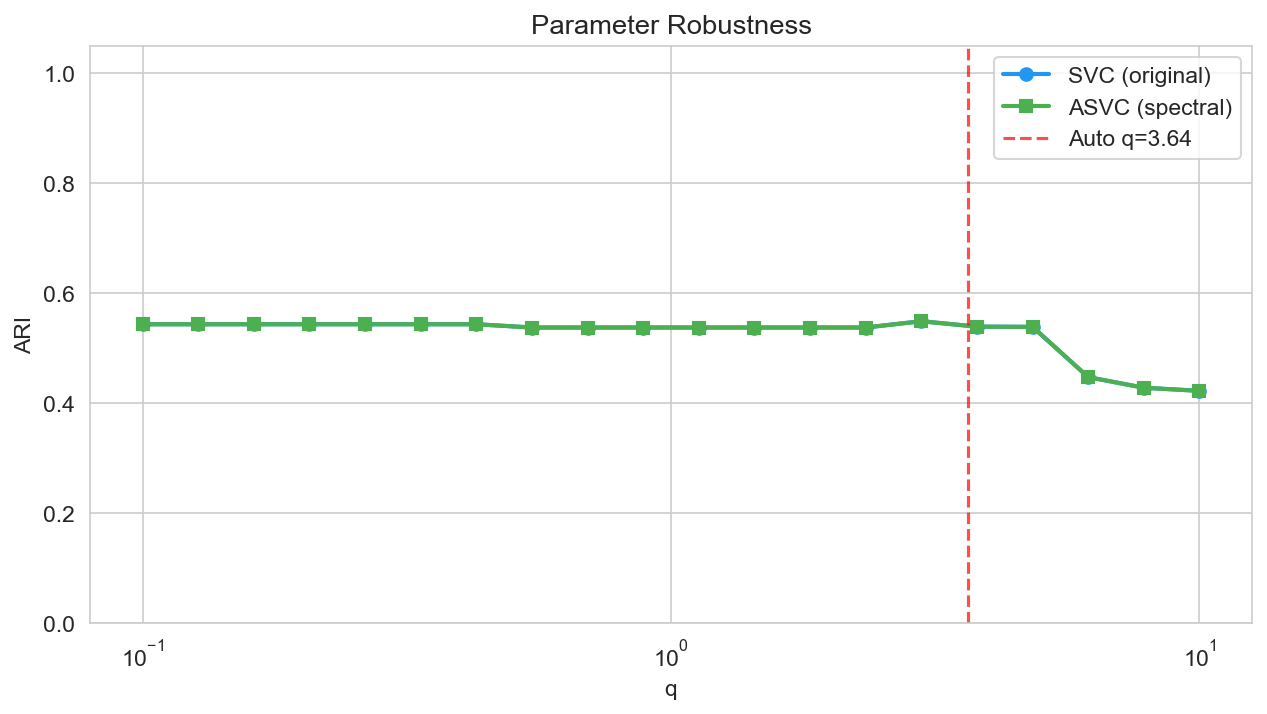
\includegraphics[width=\columnwidth]{fig/parameter_robustness.png}
\caption{Parameter robustness comparison on Iris (2D PCA). The blue curve shows SVC ARI across scanned $q$ values; the green curve shows ASVC with fixed $q$; the red dashed line marks the automatically selected $q$. ASVC's scoring function correctly identifies the high-ARI region.}
\label{fig:robustness}
\end{figure}

\subsection{Complete ASVC Algorithm}

\begin{algorithm}[t]
\caption{ASVC: Adaptive Support Vector Clustering}
\begin{algorithmic}[1]
\State \textbf{Input:} $X\!\in\!\mathbb{R}^{N\times d}$, $\nu\!=\!0.02$
\State \textbf{Output:} Cluster labels $\ell\!\in\!\{0,\dots,m\!-\!1\}^N$
\State $C\leftarrow 1/(\nu N)$
\State $[q_{\min},q_{\max}]\leftarrow\text{estimate\_q\_range}(X,k\!=\!8)$
\State $\mathcal{Q}_{\text{coarse}}\leftarrow\text{logspace}(q_{\min},q_{\max},20)$
\State $q^*\leftarrow\argmax_{q\in\mathcal{Q}_{\text{coarse}}}S(q)$
\State $\mathcal{Q}_{\text{fine}}\leftarrow\text{linspace}(0.7q^*,1.3q^*,8)$
\State $q^*\leftarrow\argmax_{q\in\mathcal{Q}_{\text{coarse}}\cup\mathcal{Q}_{\text{fine}}}S(q)$
\State $\ell\leftarrow\text{SVC}(q^*,C).\text{fit\_predict}(X)$
\State \Return $\ell$
\end{algorithmic}
\end{algorithm}

Complexity is dominated by 28 SVC invocations, totaling $O(28N^3)$. ASVC reduces the search from 2D~$(q,C)$ to 1D~$(q)$, with $\nu\!=\!0.02$ as an empirical default.
